\chapter{Comparing Devices}
To not repeat the names of the devices, the following shortening will be used: 
\begin{itemize}
    \item watch: Withings ScanWatch: \ref{section:WithingsWatch}
    \item ring: Oura ring Generation 2: \ref{section:OuraRing}
\end{itemize}
\section{Research Task}
The core application allows easy access to measurements from multiple devices in a CSV format. This enables researchers to analyse the data to answer research questions. As a supplementary project task, data analysis was performed to answer the following research question: "Do examined devices produce significantly different measurements for common fields?" Importantly, this is not the same as answering: "Are examined devices accurate?", as that would demand a much more rigorous study, requiring ground-truth measurements for every day, which are hard to acquire in practice, as those highly accurate devices are expensive, non-mobile, require technician, etc. Instead, the precision of the differences in device measurements is examined rather than the individual device's accuracy. 
\section{Data}
There are 60 days of personal data from both devices. Both devices were always worn at the same time, never one device but not the other. Both devices were configured properly - such as indicating the correct weight in both apps every week. That means that the data from devices is directly comparable. Lastly, only common measurements were used; the only non-common measurement was REM sleep duration, which the watch does not measure, so that field was deleted from the ring's rows for the analysis.
% TODO technologies in backend.
\section{Exploration}
Python with pandas, numpy and statsModels were used for analysis. To explore the dataset, a Bland-Altman plot was created on various common measurements. The difference in measurements for the same date is calculated by: $\text{ring[property]} - \text{watch[property]}$, meaning that negative values mean that the ring's measurement was lower than the watch's.
\begin{figure}
    
    \centering
    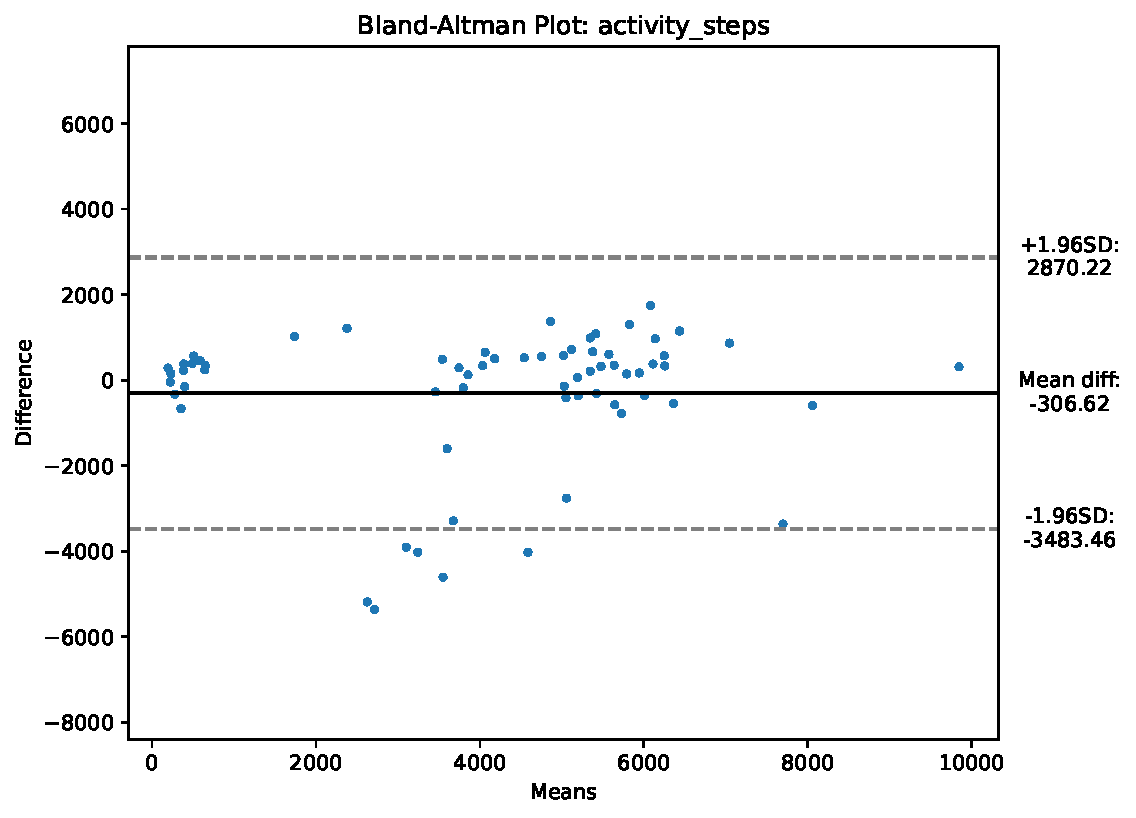
\includegraphics[width=\textwidth,keepaspectratio]{../images/bland_altman_steps.pdf}
    \caption{Bland-Altman Plot for Steps}
    \label{fig:blandAltmanSteps}
    
\end{figure}

For steps \ref{fig:blandAltmanSteps}, the average difference between devices is quite small, with the watch recording 306 more steps; for example, if the watch recorded the daily recommended number of steps - 10000, then the ring would have 9694 steps, which is only 3.06\% away from the goal. Overall, there is not a lot of variability in the differences, as points are mostly vertically clustered around the mean difference line. However, the mean difference is greatly affected by outliers, which are unlikely to occur naturally; more than a 4000 step count difference, which is more than two standard deviations away from the mean, does not make much sense and is most likely due to some error. 
\begin{figure}
    
    \centering
    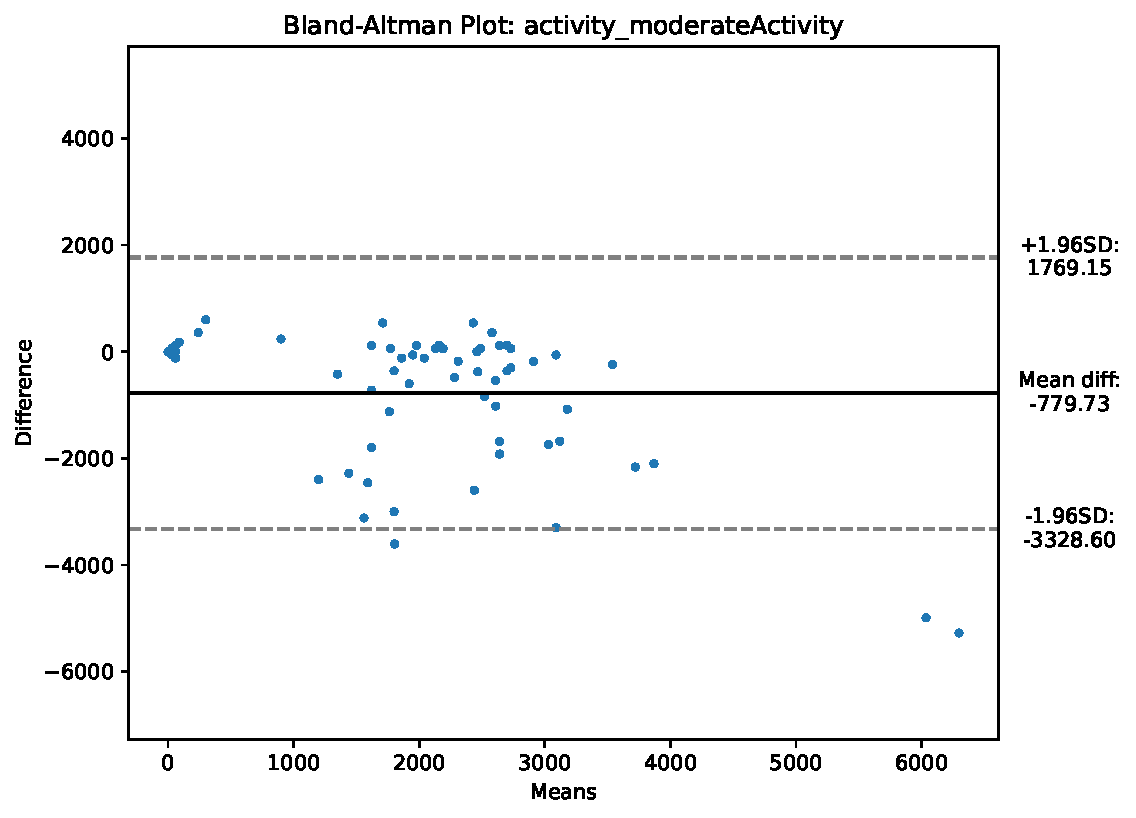
\includegraphics[width=\textwidth,keepaspectratio]{../images/bland_altman_moderateActivity.pdf}
    \caption{Bland-Altman Plot for Moderate Activity Seconds}
    \label{fig:blandAltmanSoftActivity}
    
\end{figure}

For moderate activity \ref{fig:blandAltmanSoftActivity}, the difference is more significant, with the watch on average recording 779 seconds (13 minutes) more. Although the difference might seem small, when considering how it translates into MET minutes, it has vital implications. For example, with a daily activity goal of 178 MET minutes, and using an MET factor of 3 for moderate activity, when the watch reached the goal, the ring only recorded 139 ($178 - 13 * 3$), which is 22\% away from reaching the goal; this adds up to missing 273 MET minutes in a week. Interpretation of this depends on which device is more accurate, if the watch is accurate then the ring underinflates, which is better than the other option that the ring is accurate and the watch overinflates, and of course, both could be slightly away from the true value. Assuming the ring is more accurate, users that use the watch might feel confident that they reached their activity goals to lose weight, when in fact they are missing a sizeable chunk of exercise, which could sabotage their confidence, as they might be losing less weight in reality than predicted. 

Although care has been taken to collect high-quality data, there might be user errors. Sometimes the watch could have lost contact with the skin due to a loose strap for comfortable wear, or some device turned off due to the charge running out. Also, development of the core product was still underway, so maybe some changes caused some notifications to be lost. To address outliers, z-scores are computed for each data point, and values for which: $-2 <= z <= 2$ are removed. The following are Bland-Altman plots with outliers removed for the examined properties: Steps \ref{fig:blandAltmanStepsNoOutliers} and Moderate Activity \ref{fig:blandAltmanModerateActivityNoOutliers}. The difference in step count went down to 114, which is a negligible difference, whereas the difference in the moderate activity remained relatively high at 10 minutes, suggesting some systematic difference between devices.

\begin{figure}
    
    \centering
    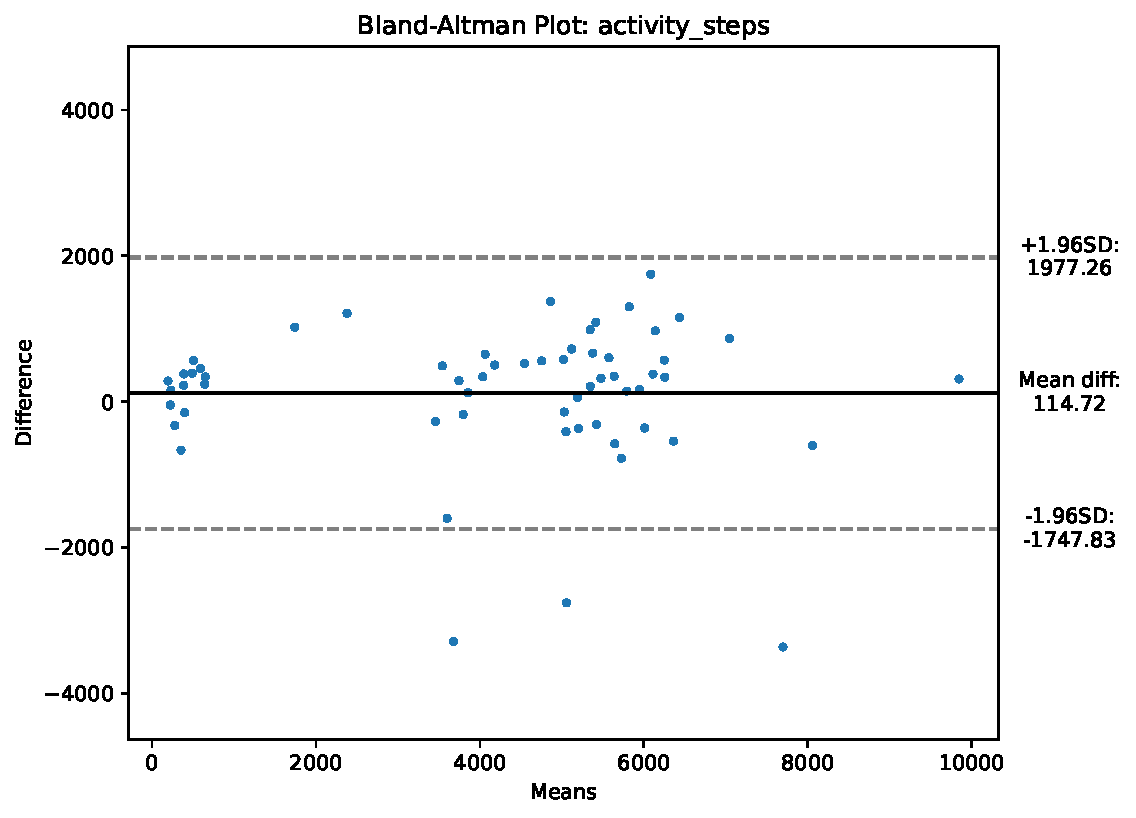
\includegraphics[width=\textwidth,keepaspectratio]{../images/bland_altman_steps_no_outliers.pdf}
    \caption{Bland-Altman Plot for Steps with previous outliers removed}
    \label{fig:blandAltmanStepsNoOutliers}
    
\end{figure}
\begin{figure}
    
    \centering
    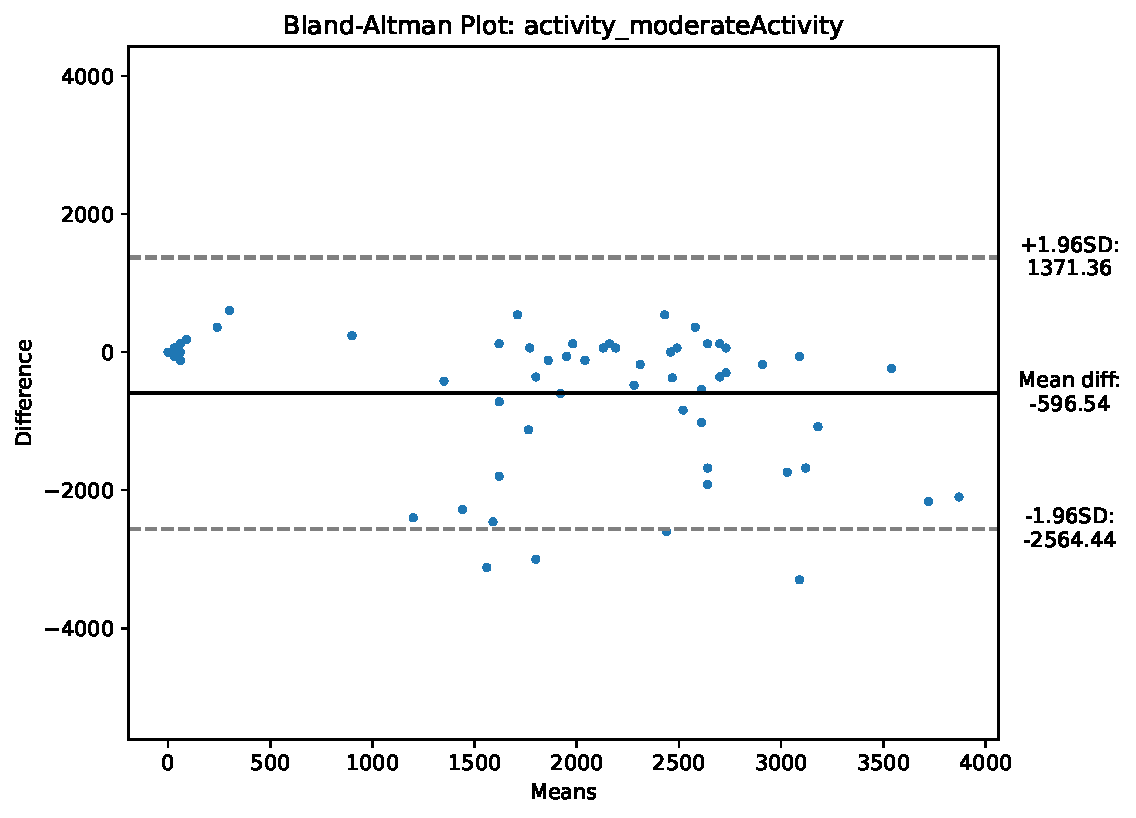
\includegraphics[width=\textwidth,keepaspectratio]{../images/bland_altman_moderateActivity_no_outliers.pdf}
    \caption{Bland-Altman Plot for Moderate Activity Seconds with previous outliers removed}
    \label{fig:blandAltmanModerateActivityNoOutliers}
    
\end{figure}
% TODO: background for bland altman, outlier detection - zscore, two one sided t-tests for equivalence bound, t-test.
\subsection{Average Percentage Difference}
The overall average difference between devices is 26.1\%, as calculated from the empirical data. Percentage differences per property: \ref{fig:empirical}. The calculation was performed as follows: 
\begin{itemize}
    \item Remove outliers using zscore.
    \item $a = \text{max}(a, 0.00001)$, $b = \text{max}(b, 0.00001)$ - prevent division by 0 errors.
    \item Calculate percentage difference: $\text{diffDate} = max(a,b) / min(a,b) \mod 1$. Modulo 1 extracts the fraction by which the larger value is bigger than the smaller one.
    \item Calculate average percentage difference: $\sum_{n=1}^{N} \text{diffDate}_n / N$.
\end{itemize}
\subsection{Statistical Testing \& Results}
Purely empirically, we could conclude that devices are different as we have a high number: 26.1\%. However, statistical significance at a certain confidence needs to be considered to make more formal conclusions. The following hypothesis testing problem was formulated for every measured property, such as steps: 

Let $\mu_1$ be the true mean of the watch's measurement of the inspected property, $\mu_2$ be the true mean of the ring's measurement of the inspected property
\begin{align*}
    H_0:\mu_1 = \mu_2 \\
    H_1: \mu_1 \neq \mu_2
\end{align*}
\begin{figure}
    
    \centering
    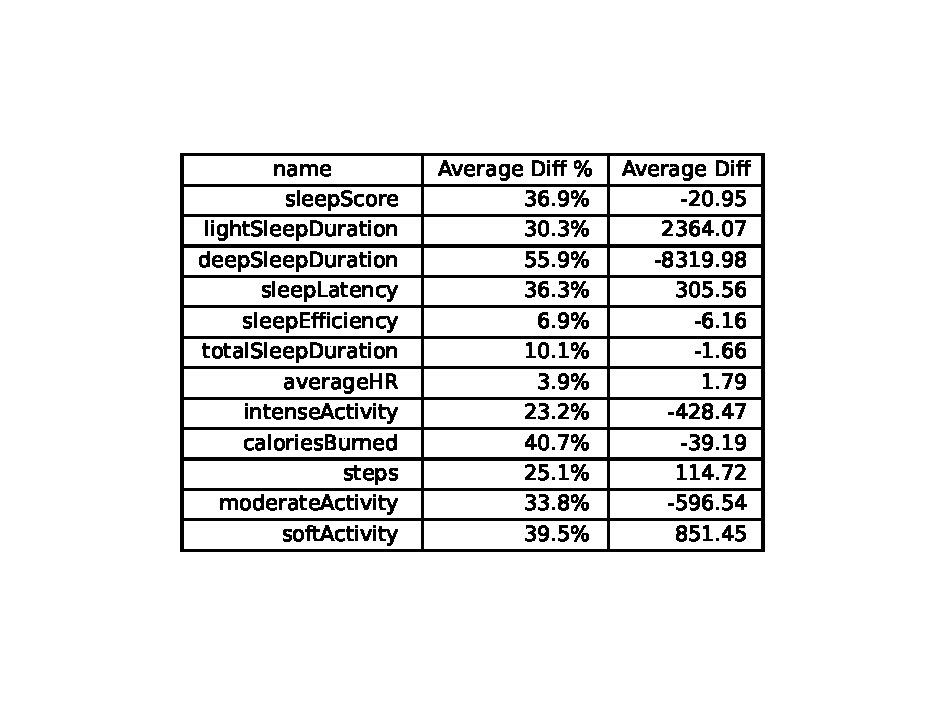
\includegraphics[width=\textwidth,keepaspectratio]{../images/empiricalResults.pdf}
    \caption{Empirical Differences Results}
    \label{fig:empirical}
    
\end{figure}

Two-tailed, Paired t-test was used to test this hypothesis. Student's t-test is preferred over Z-test because it does not require knowing the population variance, and it performs better with a smaller sample size. Paired version is used because measurements with different devices were taken from the same participant i.e. repeated measurement, which makes the measurements related. Also, equivalence bounds were calculated using TOST, which represents bounds of allowed tolerance, after which devices are equal; this is best shown via an example later on. Results: \ref{fig:results}.

\begin{figure}
    
    \centering
    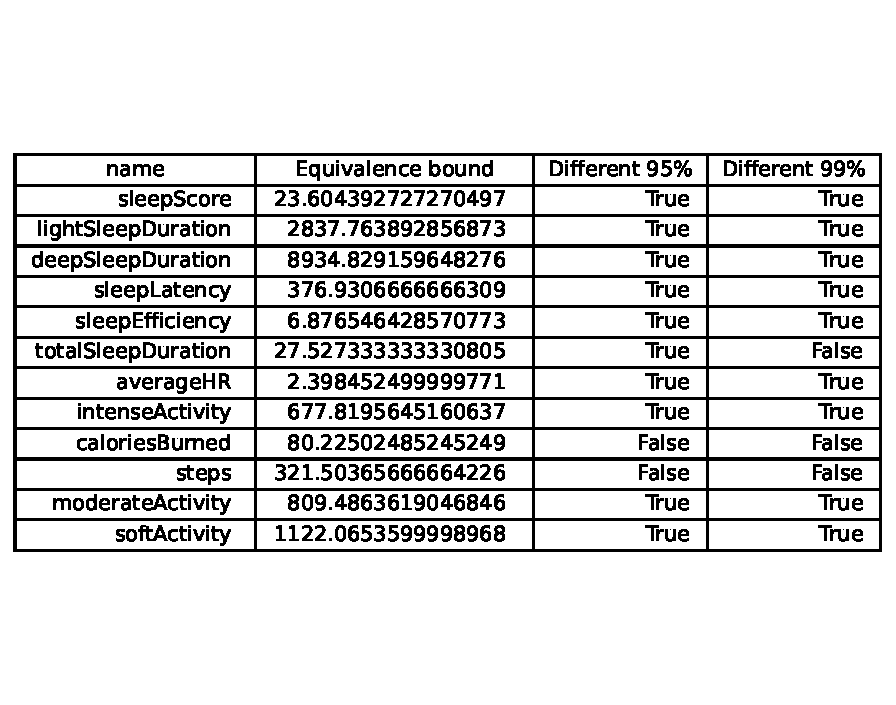
\includegraphics[width=\textwidth,keepaspectratio]{../images/results.pdf}
    \caption{Statistical Testing Results}
    \label{fig:results}
    
\end{figure}